
\chapter{运动定律}
\section{教学要求}
这一章学习动力学,讨论运动和力的关系。牛顿运动定
律是动力学的基础,这一章学习的中心内容就是牛顿运动
定律。

这一章的教学要求是:
\begin{enumerate}

\item 掌握牛顿第一定律,明确力、惯性等概念的物理意义.
\item 正确理解和掌握牛顿第二定律;掌握力学单位制;了
解超重和失重。
\item 会运用运动学公式、力的合成和分解以及牛顿运动定
律分析解决综合性问题。
\end{enumerate}

下面对这一章的教学内容作些具体说明。

运动和力的关系问题是动力学的基本问题,要建立正确
的认识又是颇不容易的,学生从日常经验出发,往往产生错
误认识,有的认识同历史上前人产生过的错误有类似之处。在
讲述牛顿第一定律之前,介绍人类对这个问题的认识过程,可
以帮助学生理解和掌握运动和力的关系。课本里介绍了伽利
略的理想实验,使学生知道伽利略是怎样得出正确结论的,并
了解在实验事实的基础进行科学思维的研究方法,以培养他
们的思维能力。

为了使教学从牛顿第一定律比较自然地过渡到牛顿第二
定律,在讲过牛顿第一定律之后,用一节教材讲述怎样使物体
的运动状态发生改变。这里,把力和运动联系起来,指出力是
使物体产生加速度的原因,加深学生对力这个概念的理解。这
一节,还讲述了质量与运动状态改变的关系,明确质量在动力
学中的意义,从而为讲述牛顿第二定律做好准备。

牛顿第二定律是这一章的重点内容。采用在教师指导下
由学生自己动手做实验,最后得出结论的做法来讲述牛顿第
二定律,可以调动学生的学习积极性和主动性,培养学生通过
实验研究问题的能力,并使学生对牛顿第二定律有深刻的
印象。

在讲述加速度和力的关系时,不可忽略它们的方向总是
一致的,这对后面研究曲线运动很重要。

以后学习匀速圆周运动、简谐振动等部分时,要学到变力
和变加速度的概念。有必要指出牛顿第二定律不仅适用于恒
力作用下的运动,而且适用于变力作用下的运动;外力随时间
改变时,加速度也随时间改变。但不要求讲述即时加速度这
个概念。

讲述力的独立作用原理,可以使学生进一步掌握在有几
个力作用时如何应用牛顿第二定律。这里,要紧的是懂得加
速度的大小和方向是由合外力决定的。

牛顿第二定律的应用有两个方面:一是已知物体的受力
情况,确定物体的运动情况;二是已知物体的运动情况,确
定物体的受力情况。利用动力学知识,知道了力和加速度,
也可以确定物体的质量。习题中带解的题目,可以使学生对
用动力学方法确定质量有所了解。

在演示实验的基础上讲述超重和失重时,涉及到弹簧秤
和被测物体组成的一个连接体。这里,只要明确研究对象是被
测物体,分析这个物体的受力情况,列出方程,再应用牛顿第
三定律,问题也就解决了。在这里既不必分别列出弹簧秤和
被测物体的动力学方程,更不要系统地讲解连解体问题。通过
超重和失重这一节的学习,还应使学生知道,某些动力学问题
常常需要综合运用牛顿第二定律和牛顿第三定律才能解决。

关于牛顿运动定律的适用范围,应要求学生有初步的了
解。限于学生的水平,这个问题不可能作深入的讨论,对于刚
体、相对论、量子力学等名词,可以只稍加说明,也不要求学生
记住这些名词。

这一章的练习和习题是按照循序渐进的原则,由浅入深,
由易到难来安排的。具体的安排是:在得出$a\propto F$和$a\propto \dfrac{1}{m}$两个公式后,安排了仅限于应用上述正比、反比关系的题目;在
得出牛顿第二定律的公式$F_{\text{合}}=ma$之后,安排了由几个力的
作用使物体产生加速度的题目;在“力学单位制”一节后面,安
排了物体受一个力作用时用动力学和运动学的知识求解的题
目;在讲完全章内容后,安排了在多个力作用下用动力学和运
动学知识求解的较复杂的综合性题目。

\section{教学建议}
这一章可分三个单元进行教学。第一单元包括引言和第
一节《牛顿第一定律》;第二单元从第二节《物体运动状态的改
变》到第七节《力学单位制》;第三单元从第八节《牛顿运动定
律的应用(一)》到第十一节《牛顿运动定律的适用范围》。

\subsection{第一单元}
在这一单元的教学中,首先可以指导学生认真阅读“历史
的回顾”这段课文,认识牛顿第一定律是怎样在伽利略理想实
验的基础上总结出来的。

\subsubsection{力不是维持运动的原因}

这一内容的教学,可以从学
生的生活经验提出所要研究的问题。譬如为了使足球不致停
下来,运动员带球前进时必须不断用脚轻轻地拨动球;又如为
了自行车不致减慢速度,总要不断地用力蹬脚踏板。让学生
带着这些问题来阅读“历史的回顾”这一段课文,然后演示教
材上图3.1的斜面对接实验(可用粗铁丝弯制成导轨来代
替对接的斜面).在演示图3.1丙的实验时,也可以使一辆
小车从斜面的一定高度上下滑后,在水平面上运动,让学生观
察在阻力比较大的水平面上,小车速度减慢得比较快,在阻力
不很大的平面上,小车速度减慢得比较慢,从而认识小车在
平面上运动所以会减慢速度,恰是由于阻力的作用,阻力的
大小不同使小车速度变慢的快慢程度也不同。同样,足球在
草地上滚动速度所以会变慢,不用力蹬脚踏板自行车所以会
减慢速度,也说明有阻力的作用,因此力不是维持运动的原
因,而是改变物体运动状态的原因。

讲清这个问题,还可以使学生体会到来自生活经验的直
观感觉不一定都是正确的,要学会用科学的思想方法去分析
现象,掌握事物发展变化的规律。

在教学中要引导学生认识伽利略的理想实验是以可靠事
实为基础的科学推论。可引导学生思考,刚才所做的演示实
验中如果水平面是光滑的,那么小车在水平面上运动时,它的
运动状态是否还会发生变化呢?小车将做什么运动?接着可以
进一步演示,使小车从斜面上滑下后在一块玻璃板上运动,可
以观察到小车运动的速度几乎没有变化,以加深对伽利略理
想实验的事实依据的认识。

\subsubsection{惯性和牛顿第一定律}

要引导学生对惯性的概念有
正确的理解。有的学生认为只有运动的物体才具有惯性;也
有的学生认为只有静止的物体才具有惯性,这些看法都是不
正确的。要使他们认识惯性是物体的固有属性,它和物体的
运动状态无关;但在力的作用下,物体运动状态改变的快慢
程度却与惯性有着直接的关系(牛顿第二定律所要研究的内
容)。而牛顿第一定律则阐明了物体的匀速直线运动状态或
静止状态都不需要力来维持,外力的作用只是改变物体的运
动状态,并不能改变物体的惯性。

\subsubsection{牛顿第一定律描述的是一种理想化的状态}

不受外
力作用的物体是不存在的。要使学生认识,即使前面所做的
演示实验中,当小车在光滑的水平面上运动时,不受任何阻
力,小车做匀速直线运动,仍然不属于牛顿第一定律所描述的
理想化状态。因为小车在水平面上运动时还受到重力和水平
面的支持力的作用,只是在水平方向上不受力,所以小车在水
平方向上的运动状态并不发生改变,牛顿第一定律所描述的
是一种理想化的状态,不同于可以用实验直接验证的牛顿第
二定律。

\subsection{第二单元}
这一单元以讲解牛顿第二定律为中心,是本章的重点。
\subsubsection{物体运动状态的改变}
教学中应该让学生认识,物体的运动状态决定于物体的
速度,根据牛顿第一定律可知,物体运动状态发生改变,必定
是外力作用的结果,为了帮助学生加深理解,可以举这样的
例子:要使静止在粗糙水平面上的物体开始运动,必须有外力
的作用,而且这个外力必须等于、大于物体与水平面间的最大
静摩擦力,物体才能改变它的运动状态,从静止开始运动;接
着,如果将所加的外力撤去,则物体只受到跟运动方向相反的
滑动摩擦力的作用,所以立即又改变它的运动状态,使运动速
度逐渐减小直到停止运动。


\subsubsection{牛顿第二定律}

为了加深对这一重要定律的理解,培
养学生用实验手段研究问题的能力,教材安排先由学生进行
实验,再由实验结果得出牛顿第二定律,在这个基础上,应使
学生认识以下几点:
\begin{enumerate}
    \item 力是使物体产生加速度的原因.加速度和力存在着
这样的关系:有力作用就有加速度产生,恒定的力产生恒定的
加速度,力发生变化,加速度随即发生相应的变化,力停止作
用,加速度立即等于零,而且不论在哪种情况下,加速度和产
生它的力的方向始终是一致的。
\item 物体运动的加速度不仅决定于外力,还同时跟物体
的质量有关,在这里,质量的大小对运动状态改变的快慢程
度起了一种制约作用,所以说质量是物体惯性大小的量度。
\item 把牛顿第二定律的实验结论$a\propto \dfrac{F}{m}$
改写成等式$F=kma$时,式中的比例常数$k$的取值跟式中其他物理量所用的
单位有关。在国际单位制中,质量$m$的单位是kg,加速度
$a$的单位是${\rm m/s^2}$, 力$F$的单位是N,于是:
\[k=\frac{F}{ma}=\frac{1{\rm N}}{1{\rm kg}\x 1{\rm m/s^2}}=1\]

这样,就可以使牛顿第二定律的公式简化为
\[F=ma\]
因此在应用牛顿第二定律公式解题时,必须使$m$、$a$、$F$三个
量都选用国际单位制单位。

\item 力的独立作用原理进一步阐明了加速度对力的依存
关系。不论物体是否还受有其他力的作用,也不论物体的初
始运动状态如何,一个力总是独立地使物体产生一个加速度。
譬如在落体运动或抛体运动中,不论是否存在空气阻力,重力
产生的加速度总是等于$g$. 也正因为这样,才能应用力的矢
量合成法则,把牛顿第二定律推广为$F_{\text{合}}=ma$, 力的独立作用
原理也为以后学习运动合成、波的叠加等知识准备了基础。
\end{enumerate}

\subsubsection{力、加速度、速度以及速度改变的关系}

加速度和力
有着直接的关系,但是物体运动的速度跟力并没有直接的关
系.学生常有如下的错误看法:
\begin{enumerate}
    \item 认为作用力大,则速度
一定大,作用力小,速度就不可能大;
\item 认为作用力如果
减小,则物体的速度也将逐渐减小。
\end{enumerate}
这两种错误都要进行
纠正。作用力大产生的加速度大,速度是否大还要取决于
初速度和加速的时间。这可以匀变速直线运动为例来加以
说明:即使加速度$a=F/m$
很大,但初速度$v_0$和加速时间$t$
如果很小,则$v_t=v_0+at$也不会很大;另一种情况,$a=F/m$
并
不大,但只要初速度$v_0$或加速的时间$t$很大,则$v_t$也不一
定小。后一种错误看法可以结合课本练习四第3题
进行讨论,指出:只要力$F$的方向和物体的初速度方向相
同,即使力$F$在逐渐减小,产生的加速度$a$也逐渐减小,但是,
物体的速度还是增的,只是每隔单位时间增加的速度$\Delta v$
在逐渐减小;直到当$F=0$, $a=0$时,物体的速度就不再增
大,物体将以做变速运动时最大的末速度为速度做匀速直线
运动。关于这道题目还可用一个比喻来加以说明:如果往银
行存钱,每个月存入的钱数在逐渐减少,但存款数还是在增
加的。

\subsubsection{关于质量和重量的区别与联系}

在物理学的传统讲
法中,质量和重量是两个不同的概念,质量就其本身的含义来
说,就是组成物体的物质多少;从动力学的观点来看,是物体
惯性大小的量度。质量是标量,物体的重量则是指物体所受到
的地球的重力,是矢量。

课文中先后出现的两个式子$G=mg$和
$\dfrac{G_1}{G_2}=\dfrac{m_1}{m_2}$
表明了质
量和重量的联系。教学时对这两个式子的意义可掌握以下的
分寸:
\begin{enumerate}
    \item $G=mg$这一关系式,在初中把比值$g$作为一个比例
常数,$g=9.8{\rm N/kg}$。它的意义是质量为1千克的物体的重
量是9.8牛顿.而高中课本则是从牛顿第二定律$F=ma$推导得出的,这是指物体在重力作用下运动时,重力产生的加
速度为$g$, 物体的质量为$m$, 则物体所受的重力$G=mg$. 两
处对$G=mg$的讲法,着眼点不同,但含义是一致的。

\item $\dfrac{G_1}{G_2}=\dfrac{m_1}{m_2}$一式所表明的意义是在地球上同一地点,物体的重量正比于物体的质量。这就是说,在地球上同一地点,
一切自由落体的加速度$g$都相等,在重力作用下,$g$的大小和
方向都是确定的。即比值$g=G/m$
是与物体的质量$m$无关的
一个量。

\item 由于现在已经规定重量作为质量的同意词,不再用
来表示物体所受的重力。因此,今后中学物理教学中如何处
理有关重量的问题,尚须进一步研究。
\end{enumerate}

\subsection{第三单元}
这一单元主要是综合应用牛顿运动定律和运动学的知识
来解决一些实际问题,并了解什么是超重和失重现象,解牛
顿定律的适用范围。

\subsubsection{牛顿运动定律的应用}

教材的安排是先通过应用
(一)讨论从物体的受力情况确定物体的运动情况;再通过应
用(二)从物体的运动情况确定物体的受力情况,要引导学生
认识在分析实际问题时,这两个方面常常是结合使用的,而对
运动物体受力情况的分析则是解决任何力学问题的基本出
发点。

\subsubsection{物体受力分析}

在对物体进行受力分析时,要让学生
注意首先应明确研究的对象,考察研究对象和周围哪些物体
有联系,并要结合物体的运动状态来分析。这是分析物体受
力情况时的一条基本思路,譬如在分析课本126页例题2
时,应向学生指出:题目是要求线对小球的拉力,因此小球应
是研究的对象;跟小球发生联系只有地球和悬线两个物体,也
就是小球只受到重力和悬线拉力这两个力的作用。既然小球
跟随小车一起做匀变速运动,则小球所受的合力必然不等于
零,而且小球运动的加速度必定是由重力和悬线的拉力的合
力所产生,又由于小球是沿着水平方向做匀变速直线运动,所
以这一合力也必定是沿着水平方向。于是就可以按课本图
3.11所示进行力的合成.由于合力所产生的加速度已由题
目给出,所以就可计算出悬线对小球的拉力。

\subsubsection{超重和失重} 在讲解超重和失重现象时,可以让全体
学生利用弹簧秤做课本图3.12的实验(弹簧秤可用
量程为250克力或400克力的,物体可用100克或200克的
钩码)。

在弹簧秤静止的情况下,观察指示器所指的读数就等于
钩码的重量。使弹簧秤急剧上升,就可以看到弹簧秤指示器
所指的读数突然增大,但随即又减小了,要指导学生观察开
始上升时弹簧秤读数增大这一变化。为了看清楚这一点,可
以让学生在弹簧秤挂了钩码静止的情况下,用一小块纸片卡
在弹簧秤指示器的下面,当弹簧秤加速上升时,指示器下降将
会把纸片推到下面读数较大的位置上。这样,当弹簧秤静止
时就可以看出弹簧秤读数曾经增大到多大了。

同样,在观察物体的失重现象时,应指导学生观察当弹簧
秤突然加速下降时读数减小的现象。为了观察读数曾经减小
到什么程度,也可用一小纸片卡在弹簧秤指示器的上端,用
以记录失重时的读数。

在分析超重和失重现象时,应指出:

\begin{enumerate}
    \item 挂在弹簧秤下的砝码只受重力和弹簧拉力的作用,
当钩码在竖直方向上做变速运动时,重力和拉力的合力不可
能等于零。这一合力就是使钩码产生加速度的力。在钩码向
上做加速运动或向下做减速运动时,所需的合力方向都是向
上的,而重力的方向是竖直向下的,因此只有依靠弹簧秤的拉
力大于重力,才能使得合力方向向上。这样,弹簧秤的读数就
会大于钩码的重量,这就是产生超重现象的原因,而当钩码
向下做加速运动或者向上做减速运动时,所需的合力的方向
向下,跟物体重力方向一致,因此重力中的一部分就用来产生
向下的加速度。由于重力“用掉”一部分,因此钩码作用于弹
簧秤的力将减小,即弹簧秤的读数将减小,这就是产生失重现
象的原因。
\item 如果物体向下做加速运动的加速度等于$g$, 则物体
的重力将全部用来产生加速度,这样就没有多余的力作用于
弹簧秤,弹簧秤的读数应等于零。

可以由教师做一演示,将挂有重物(钩码)的弹簧秤用线
悬在高处,在弹簧秤的指示器上贴一小块白胶布以便于观察,
这时弹簧秤的读数等于重物的重量。当用火柴烧断悬线后,
重物和弹簧秤一起自由下落,在这过程中可以观察到弹簧秤
的读数立即减小到零(演示时在落地处准备好一个网兜以承
接弹簧秤使之不会摔坏)。指出这是完全失重的现象。

\item 要使学生明确,不论超重还是失重现象,物体所受到
的重力是没有变化的,只是在物体静止时,支承这个物体的另
一物体(如桌面、悬线等)发生形变,产生了弹力作用于物体,
使物体保持平衡。当物体加速下降时,由于重力中的一部分用
来产生向下的加速度,物体需要的支持力变小了。相反,物体
加速上升时,物体所受的重力虽然也没有变化,但重力并不能
产生向上的加速度,因此支持物提供的弹力除了克服物体的
重力外还要包括使物体产生向上加速度所需的力,因而支持
物的弹力将增大,所以通常用弹簧秤(测力计)来测量物体的
重量时,必须使物体处于静止状态,避免失重或超重的影响。
\end{enumerate}

\subsubsection{牛顿运动定律的适用范围}

只需简单地向学生介绍,
牛顿定律只适用于解决低速运动问题,而不能适用于研究高
速运动,对于微观粒子的运动,一般说来,牛顿力学也是不
适用的。可指出所谓高速是指粒子的速率已高达可与光速相
比拟的程度。关于爱因斯坦狭义相对论的时空观,只需大致
地根据课本所叙述的内容进行介绍,不必作深入的讲解。这
节教材的意图在于一方面扩大学生的知识面,更重要的是使
学生认识到任何规律都有它的适用范围。

\section{实验指导}
\subsection{演示实验}

\subsubsection{阻力是使物体运动变慢的原因}
小车自斜面滑下后在水平面上运动的演示实验,可用宽
约12—15厘米、带有档边(高约0.8—1.0厘米)的两段木板,
分别作为斜面和水平面拼接起来,作为斜面的木板长约60厘
米,作为水平面的木板长约120厘米.在水平长木板的一端
装一个用扁铁作边框的网兜,如图3.1所示.长木板平面上
贴上塑料装饰板,在上面平铺一层软棉布(灯芯绒或绒布),棉
布上面再铺放两层毛巾布,以增大阻力。将作为斜面的木板
的一端用木块垫起,倾角$5^{\circ}$左右.要注意斜面跟长木板平面
的拼接处要尽可能吻合。
\begin{figure}[htp]
    \centering
    \includegraphics[scale=.6]{fig/3-1.png}
    \caption{}
\end{figure}

实验时将小车放在斜面顶端由静止开始释放。小车到达
铺有毛巾布的平面上后,运动30厘米左右即停下来;然后把
两层毛巾布取下(注意用薄木片调节拼接处的高度使之吻合),
再把小车放在斜面顶端由静止开始释放,小车在铺有软棉布
的平面上运动的距离将增大到60厘米左右.如果把棉布取
下,小车在斜面的同一高度滑下后,可以沿着塑料平面一直运
动下去直到落入网兜里。

\subsubsection{用气垫导轨观察骑块的运动}
使用前必须将导轨调节水平(沿导轨方向和垂直于导轨
方向都应用水平仪进行调节)。用软布擦去骑块内侧以及导
轨表面的浮灰。然后接通气泵,如发现气孔有堵塞现象,可用
细铜丝(从多芯软导线中抽出一根使用,不要用钢丝,因为钢
丝太硬会使气孔边缘卷口起毛,增大骑块运动时的阻力)通一
下,务必使每个气孔保持畅通。

实验时应先开动气泵,待正常供气后,再将骑块放上导
轨,轻轻推动一下,便可观察到骑块的运动很接近于匀速直线
运动。应强调指出,所要观察和研究的是骑块已经开始运动
以后的一段过程,由于摩擦阻力很小可以忽略,重力和气垫的
托力相互平衡,合力为零,因此骑块的匀速直线运动状态并不
发生改变,当骑块到达导轨一端被弹簧片弹回反向运动时,可
指出这时由于受到外力作用,迫使骑块改变了运动方向(也就
是改变了运动状态),但在反向运动的过程中,由于骑块所受
合力为零,骑块的匀速直线运动状态仍不发生改变。

\subsubsection{惯性现象}
如图3.2所示,将小车(质量约为200克)用细线通过定滑
轮和一质量较大的钩码(譬如30克)相连,用手挡住小车,不使
它运动,将一木块(体积约为$3\x6\x10{\rm cm^3}$)竖起来放在车上。
释放后,小车突然做加速运动,木块由于惯性将向后面倾倒。
\begin{figure}[htp]
    \centering
    \includegraphics[scale=.6]{fig/3-2.png}
    \caption{}
\end{figure}

利用同一装置继续演示,开始时用手扶住木块同时施加
适当的阻力使小车的加速度不至太大。待小车和木块一起运
动后再完全放手,这时木块和小车将保持相对静止,当小车
运动到平面一端受阻突然停止运动时,木块由于惯性将向前倾倒。

\subsubsection{物体运动状态的改需要力的作用}
物体速度大小的改变.将一辆小车放在水平的玻璃
板上,使小车从静止到运动需要用手推,这就是要有力的作用
(图3.3);在小车已经具有速度的情况下,要使它停止运动,
需要用手来挡,这也就是要有力的作用,如图3.4。
\begin{figure}[htp]
    \centering
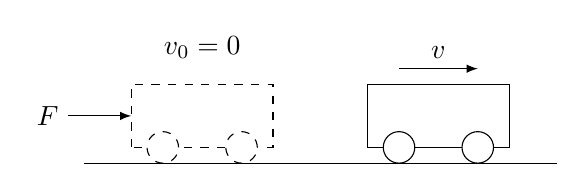
\begin{tikzpicture}[>=latex]

    \node at (.5,1)[above]{$v_0=0$};
\draw[->](3,1)--node[above]{$v$}(4,1);
    \draw(2.6,0)rectangle (4.4,.8) ;  
\draw[dashed](-.4,0)rectangle (1.4,.8) ;   
  \foreach \x in {0,1}
{
    \draw[fill=white, dashed] (\x,0) circle(.2);
    \draw[fill=white] (\x+3,0) circle(.2);
}  
\draw[->](-1.2,.4)node[left]{$F$}--(-.4,.4);
\draw(-1,-.2)--(5,-.2);
\end{tikzpicture}
    \caption{}
\end{figure}

\begin{figure}[htp]
    \centering
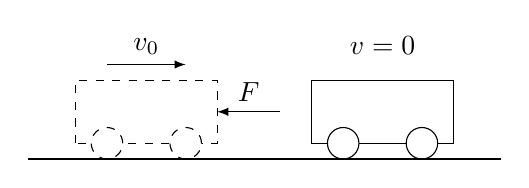
\begin{tikzpicture}[>=latex]
    \node at (3.5,1)[above]{$v=0$};
    \draw[->](0,1)--node[above]{$v_0$}(1,1);
    \draw(2.6,0)rectangle (4.4,.8) ;  
\draw[dashed](-.4,0)rectangle (1.4,.8) ;   
  \foreach \x in {0,1}
{
    \draw[fill=white, dashed] (\x,0) circle(.2);
    \draw[fill=white] (\x+3,0) circle(.2);
}  
\draw(-1,-.2)--(5,-.2);
\draw[->](2.2,.4)--node[above]{$F$}(1.4,.4);
\end{tikzpicture}
    \caption{}
\end{figure}

物体速度方向的改变。将一瓷球(白色的、半径较大,
可见度较大,或者用灌水的乒乓球)系在细线一端,另一端有
一金属小杯,把环套在竖直方向的固定轴上,给瓷球一个垂直
于拉线方向的速度,球就在水平面上沿着一个以线长为半径
的圆周运动,如图3.5所示(水平面可以用涂塑装饰板做).如
果水平面的阻力很小,可以认为瓷球的速率不变,但是从拉线
被绷紧的现象可以想象,线对瓷球有拉力的作用,才使瓷球的
运动方向时刻发生改变。
\begin{figure}[htp]\centering
    \begin{minipage}[t]{0.48\textwidth}
    \centering
    \includegraphics[scale=.8]{fig/3-5.png}
    \caption{}
    \end{minipage}
    \begin{minipage}[t]{0.48\textwidth}
    \centering
    \includegraphics[scale=.8]{fig/3-6.png}
    \caption{}
    \end{minipage}
    \end{figure}

物体的速度大小和方向都发生改变,如图3.6所示,
使一乒乓球沿着桌面以某一速度运动,当乒乓球离开桌子后
将沿一曲线下落。可以这样设想:乒乓球离开桌子后,如果没
有重力的作用,仍将沿着原来的水平方向作匀速直线运动。
正是由于下落过程中只受到重力的作用,乒乓球的速度大小
和方向才都发生了改变。

\subsubsection{加速度和力的关系以及加速度和质量的关系}
(演示方法见学生实验8和9)

\subsubsection{牛顿第二定律的应用}
为结合课本126页例题2的讲解可以做如下的演示:
用手提着一个挂在细绳一端的质量较大的单摆球,当球静止
时,细绳在竖直方向,当提着小球突然向右侧加速跑动时,即
可看到悬挂小球的线向左偏斜的现象。

\subsubsection{超重和失重现象}

可按课本图3.12所示的情况
进行演示,为了能把超重和失重的最大续数
固定下来,可以剪两小块厚纸(如用包装牙膏
等软管用纸盒),形状如图3.7所示.两侧狭
缝的宽度相当于弹簧秤刻度板的厚度,当弹簧秤挂着100
克钩码时,把纸片卡在弹簧秤指示器的下方和上方。卡入纸
片时,先将纸片顺着刻度板中部的隙缝嵌人,然后再扭转$90^{\circ}$,
并使它紧靠着指示器。当把弹簧秤迅速上提或迅速下降时,指
示器就会把纸片推向下方或上方,并停留在那里,这样就可
以看出超重和失重的最大读数。
\begin{figure}[htp]\centering
    \begin{minipage}[t]{0.48\textwidth}
    \centering
    \includegraphics[scale=.8]{fig/3-7.png}
    \caption{}
    \end{minipage}
    \begin{minipage}[t]{0.48\textwidth}
    \centering
    \includegraphics[scale=.6]{fig/3-8.png}
    \caption{}
    \end{minipage}
    \end{figure}

如图3.8所示,将一杠杆支放在铁架台上,在杠杆左
端悬挂一根细链条,使链条的
一端$A$固定在杠杆上,另一端
$B$用细线系在链条$A$端的一
个环上,在杠杆右端挂一砝码
使杠杆平衡。点燃火柴烧断系
住链条$B$端的细线,使这一半
链条下落。这时可观察到杠杆
左端向上倾斜,说明杠杆左侧的一半链条下落时发生了失重现象。这是因为当这一半链条
下落时,它所受的重力已用于产生向下运动的加速度,作用于
杠杆上的力减小了,因此杠杆失去了平衡,但当这一半链条
下落到被上一半链条拉住时,则杠杆又会恢复平衡。

\subsection{学生实验}
\subsubsection{研究加速度和力的关系}
实验时要注意以下几个问题:

实验前要消除摩擦阻力的影响,将长木板不带定滑
轮的一端下面垫放一木块,使木板倾斜(约$5^{\circ}$左右),将小车
放在木板上,先不要拴上砂桶。在小车后面固定一条纸带,并
让它穿过打点计时器的两个限位孔,将小车释放后,它可能
仍保持静止,也可能沿长木板加速下滑。适当改变木块的垫
放位置(即改变木板的倾斜程度),直到推动一下小车后,小车
基本上能匀速下滑(纸带上打出的点子的间隔基本上是均匀
的)。这时摩擦阻力和小车的重力沿斜面方向的分力相平衡,
消除了摩擦的影响。

砂桶和砂的质量只有远小于小车质量($m\ll M$)的条
件下,才可以认为它的重量(mg)等于对小车的拉力(还要注
意调节定滑轮的位置使得拉绳平行于斜面),一般实验用的
小车质量约为200克,因此砂和砂桶的总质量以不超过20克
为宜。如果砂桶和砂的质量太大将会产生明显误差(系统误
差)。这个问题不要在实验时讨论,以免分散学生的注意力,
可以在总结出牛顿第二定律以后再安排讨论。

这个实验中,拉力所用的单位,可以用弹簧秤直接测
量砂桶和砂的重量,然后读取用牛顿做单位的读数。

每次改变拉力,打出的纸带都要进行编号,并标明所
用拉力的大小,以免在处理数据时发生张冠李戴的混乱
情况。

在指导写实验报告时,应要求学生把每次改变拉力
时的记录纸带,作为原始资料附在实验报告中。并要写出自己
设计的能够反映数据处理过程的表格,以及与之相应的、画在
坐标纸上的$a$-$F$图象。实验报告还应包括明确的实验结
论.在最后部分还可根据课本练习二第2题的要
求,利用实验数据来求出每次实验中,加速度$a$和拉力$F$的
比值,看看它们是否大致相等,可启发学生思考这一比值跟
$a$-$F$图象中直线的斜率有怎样的关系?

\subsubsection{研究加速度和质量的关系}
这个实验的注意事项和编写实验报告的要求和实验(一)相
同。此外还应注意,在改变物体质量时,变化范围可适当放大
一些,如可分别增加50克、100克、150克、200克、250克
砝码。

实验后可引导学生讨论课本练习三第2、3题.

\section{习题解答}

\subsection{练习一}
\begin{enumerate}
	 \item 一个球以20${\rm cm/s}$的速度运动着,而且没有受到力的作用,5秒后它的速度将是多大?
	 
     \begin{solution}
        运动着的球没有受到力的作用,它将保持匀速直线
        运动状态,所以5秒后仍以20${\rm cm/s}$的速度沿着原来运动
        的方向做匀速直线运动。
     \end{solution}
	 \item 在行驶的火车里的水平桌面上放着一个小球,当小球突然相对于车厢发生向前运动或者向后运动时,火车的运动状态分别发生了怎样的改变?
	 
     \begin{solution}
        当小球突然相对于车厢发生向前运动时,说明火车
        突然制动做减速运动;当小球突然相对于车厢发生向后运动
        时,说明火车突然加速做加速运动。
     \end{solution}
	 \item 地球从西向东转,为什么我们向上跳起来以后还落到原地,而不落到原地的西边?
	 
     \begin{solution}
        因为我们站在地面时具有和地面相同的自转速度,
        当我们向上跳起时,由于惯性,在水平方向上仍要保持原来的
        速度前进,因此落下时仍落在原地而不会落到原地的西边。
     \end{solution}
	 \item 分别举出几个利用惯性和防止惯性的不利影响的例子.
	 
     \begin{solution}
        这类例子很多。锤头和木柄间有些松动,可以把锤
        子竖起来使锤柄朝下,在固定物体上撞击几下,锤柄因撞击受阻而突然停止运动,锤头由于惯性要继续向下运动,结果锤头
        和柄就套紧了。这是利用惯性的例子。为了行车安全,规定
        了城市里各种车辆的最高行驶速度,这是为了在紧急制动时
        防止由于惯性而造成的事故,这是防止惯性的不利影响的
        例子。
     \end{solution}
\end{enumerate}



\subsection{练习二}
\begin{enumerate}
	\item 根据你的记录纸带,量出有关数值,计算出每次实验的加速度,列出表格,作出$a-F$图象.
	 
    \begin{solution}
        说明:本题应根据每个人的实验结果,处理数据,填写表
        格,作出图象。
    \end{solution}
	\item 利用你自己的数据算出每次实验中$a$和$F$的比值,看看这些比值是否大致相同?利用这种办法来研究$a$和$F$的关系,比起用图象来研究,哪种办法方便?
	 
    \begin{solution}
        说明:根据每次实验中$a$和$F$的对应数据计算出来的$a$
        和$F$的比值,大致是相同的。用这种办法虽然也可以得出加
        速度$a$和力$F$成正比关系的结论,但是要进行多次计算。而
        用画$a$-$F$图象的方法,可以看出各个点基本上分布在同一条
        通过坐标轴原点的直线上,这样就可以方便地得出$a$和$F$成
        正比关系的结论。因此采用图象来研究比较方便。  
    \end{solution}
	\item 5牛的力的作用在一个物体上,能使它产生2$\msq$的加速度,要使它产生5$\msq$的加速度,需要多少牛的力?
	 
    \begin{solution}
对于一个确定的物体来说,加速度和力成正比。  
\[\frac{a_1}{a_2}=\frac{F_1}{F_2}\]
所以:
\[F_2=\frac{F_1a_2}{a_1}=\frac{5\x5}{2}=12.5{\rm N}\]      
    \end{solution}
\end{enumerate}



\subsection{练习三}
\begin{enumerate}
	\item 根据你的记录纸带,量出有关数值,计算出每次实验的加速度,列出表格,作出$a-1/m$图象.
	 
    \begin{solution}
        说明:本题应根据每个人的实验结果,处理数据,填写表
格,作出图象。
    \end{solution}
\item 利用你自己的数据算出每次实验中$m$和$a$的乘积,
看看乘积的数值是否大致相同?你由此能得出什么结论?利用这种办法来研究$a$和$m$的关系,比起用图象来研究,哪种办法方便?
	 
\begin{solution}
    说明:根据每次实验中$m$和$a$的乘积,可以看出它们的
数值大致是相同的。这说明了在相同的力作用下,小车的加
速度$a$和小车的质量$m$成反比。利用这种办法来研究$a$和$m$
的关系要进行多次计算,用图象法研究,也要多次计算$1/m$
的数值,但画出$a$-$1/m$图象后,可以直观地看出各个点基本
上分布在同一条通过坐标轴原点的直线上,说明$a$和$1/m$成
正比,从而得出$a$和$m$成反比关系的结论。

因此在研究加速度和质量的关系时,这两种处理数据的
方法对比起来,用图象法并不显得很方便,但是作为一种数据
处理方法还是应该学习的。
\end{solution}
\item 你已经用图象研究了$a$和$F$、$a$和$m$的关系,谈谈用图象处理实验数据的好处.
	 
\begin{solution}
利用图象比较直观,能为我们寻求物理量之间的定量关系提供线索,譬如$a$-$F$图象是一条直线,这就直观地说
    明了$a$和$F$成正比关系.$a$-$1/m$图象也是一条直线,说明了
    $a$和$1/m$成正比即$a$和$m$成反比关系.

    此外,图象法的优点还在于对测量数据的取舍比较方便。
    譬如在画$a$-$F$图线时,有些点并不在直线上,但只要直线能
    通过大多数的点,就可以得出$a$和$F$成正比的结论。而如果
    要计算每一次实验中$a$和$F$的比值,有的比值可能跟真实值
    相差较大,这样求得的平均比值的误差就会偏大。    
\end{solution}
\item 一辆卡车在空载时质量是$3.5\times 10^3$千克,载货时的质量是$6.0\times 10^3$千克用同样大小的牵引力,如果空载时使卡车产生1.5$\msq$的加速度,载货时产生多大的加速度?(不考虑阻力)
	 
\begin{solution}
    在不考虑阻力的情况下,对卡车的牵引力就是使卡
车产生加速度的力,在同样大小的牵引力作用下,卡车的加速
度跟它的质量成反比。
\[\frac{a_1}{a_2}=\frac{m_2}{m_1}\]
所以:
\[a_2=\frac{m_1a_1}{m_2}=\frac{3.5\x 10^3\x 1.5}{6.0\x 10^3}=0.88\msq\]
\end{solution}
\end{enumerate}



\subsection{练习四}
\begin{enumerate}
	\item 从牛顿第二定律知道,无论怎样小的力都可以使物体产生加速度,可是我们用力提一个很重的物体时,却提不动它.这跟牛顿第二定律有无矛盾,为什么?
	 
    \begin{solution}
        没有矛盾。在用力提一个很重的物体时,没有提起来,这是因为所用的力小于物体所受的重力。用力的结果只
能减小重物对支持物的压力,重物虽然受到向下的重力,向上
的支持力以及手提重物时的作用力,但它所受的合力还是等
于零,因此重物不会产生加速度,自然就继续保持静止状态
不动。
    \end{solution}
\item 要把一个箱子在地板上从这一端推到另一端,我们在全部时间内都必须用力推它,停止用力,箱子就会停下来.马必须用力拉车,车子才前进,停止用力,车子就会停下来.亚里士多德怎样解释上述现象?根据牛顿运动定律应该怎样解释?
	 
\begin{solution}
    亚里士多德认为,力是维持物体运动的原因。必须
    有力作用在物体上,物体才能运动,没有力的作用,物体就要
    静止下来,根据这种观点,人必须用力推箱子,箱子才能运动,
    停止对它用力,它就停下来;马必须用力拉车,车才能运动,停
    止对它用力,它就停下来。

    根据牛顿运动定律,力不是维持运动的原因,而是改变物
    体运动状态的原因。当人的推力大于箱子和地板间的摩擦力
    时,箱子就会在合外力的作用下产生加速度改变原来的静止
    状态开始运动;当人停止用力时,箱子又会在摩擦阻力的作用
    下产生跟原来的运动方向相反的加速度,使它做减速运动,很
    快地停了下来,马拉车,车子会前进,停止用力,车子就会停
    下来的原因,也是如此。
\end{solution}
\item 一个物体受到一个逐渐减小的力的作用,力的方向跟速度的方向相同,物体的速度怎样改变?
	 
\begin{solution}
    物体的速度将逐渐增大,直到这个力减小到零为止。这是因为虽然力在逐渐减小,只是使物体产生的加速度逐渐
    减小,但由于力的方向跟速度的方向相同,它的速度还是不断
    增大的。
\end{solution}
\item \begin{enumerate}
\item  质量是0.5千克的物体在一个恒力的作用下得到
0.1$\msq$的加速度,这个恒力是多大?
\item 10牛的力使一个物体得到2.0$\msq$的加速度,这个物体的质量是多大?
\item 质量是0.1千克的物体,在5牛的恒力作用下,得到多大的加速
度?
\end{enumerate}
	 
\begin{solution}
    根据牛顿第二定律
\begin{enumerate}
    \item $F=ma=0.5\x 0.1=0.05{\rm N}$
    \item $F=ma,\quad m=\dfrac{F}{a}=\dfrac{10}{2.0}=5{\rm kg}$
    \item $F=ma,\quad a=\dfrac{F}{m}=\dfrac{5}{0.1}=50\msq$
\end{enumerate}
\end{solution}
 \item 质量是1.0千克的物体受到互成30$^\circ$角的两个力的
作用,这两个力都是10牛,这个物体产生的加速度是多大?
	 
\begin{solution}
    这个物体所受到的合力
\[F_{\text{合}}=2F\cos\frac{\alpha}{2}=2\x 10\x \cos15^{\circ}=2\x 10\x 0.966=19.3{\rm N}\]
根据牛顿第二定律合力产生的加速度
\[a=\frac{F_{\text{合}}}{m}=\frac{19.3}{1.0}=19.3\msq\]
\end{solution}
\item 下列说法是否正确:
\begin{enumerate}
\item 物体的速度越大,表明物体所受的合外力越大.
\item 根据$F_{\text{合}}=ma$,得到$m=F_{\text{合}}/a$,所以物体的质量跟物
体所受的合外力成正比.
\item 物体所受合外力越大,速度变化越大.
\end{enumerate}

\begin{solution}	 
\begin{enumerate}
    \item 不正确。因为物体的速度大小和合外力的大小并
    无直接关系,合外力只决定了物体的加速度。
    \item 不正确。因为质量是物体惯性大小的量度,是物体固
    有的属性,跟物体是否受力无关。
    \item 不一定正确。因为速度变化$\Delta v$的大小不仅跟合外力
    产生的加速度$a$有关,还跟速度发生变化的时间$\Delta t$有关,即
    $\Delta v=a\Delta t$. 即使物体所受的合外力增大了,如果作用时间
    $\Delta t$很小,速度的变化$\Delta v$也不一定大。
\end{enumerate}
         
\end{solution}

\end{enumerate}








\subsection{练习五}
\begin{enumerate}
\item 先后在广州和北京用天平来称量同一个物体,得到
的结果是否相同?如果先后用弹簧秤来称量,得到的结果是否
相同?说明理由.
	 
\begin{solution}
    天平是利用杠杆(并且是等臂杠杆)平衡原理来称量
物体质量的,设被测物体的质量为$m_x$, 砝码质量为$m$, 力臂
为$L$, 当天平平衡时,应有$m_xgL=mgL$的关系。消去力臂$L$
和重力加速度$g$, 则$m_x=m$. 因此先后在广州和北京用天平
来称量同一个物体,得到的结果是相同的。

而弹簧秤是根据在弹性限度内,弹簧的形变跟弹力成正
比的原理制成的。作用的力越大,则弹簧的形变量也越大,弹
簧秤的示数也越大。用弹簧秤来测量物体的重量$G=mg$时,
由于广州的重力加速度小于北京的重力加速度,所以如果先
后用弹簧秤来称量,得到的结果是不相同的,在广州称量时弹簧秤的示数要小些。
\end{solution}
\item 一个学生认为半块砖的重力加速度是整块砖的重力
加速度的两倍,因为半块砖的质量是整块砖的质量的一半.另
一个学生认为半块砖的重力加速度是整块砖的重力加速度的
一半,因为半块砖的重量是整块砖的重量的一半.他们的说
法对不对?为什么?
	 
\begin{solution}
    他们的说法都不对,这是因为半块砖整块砖的重
力加速度$g$在同一地区是不变的。第一个学生的错误在于认
为半块砖和整块砖受到的重力是相等的;另一个学生的错误
在于认为半块砖和整块砖的质量是相等的,而他们发生错误
的共同原因还在于都认为重力加速度对于不同的物体可以是
不同的。
\end{solution}
\item 北京的重力加速度为980.1${\rm cm}/{\rm s^2}$.质量是1千
克的物体在北京的重量是多少牛?
	 
\begin{solution}
    根据重量和质量的关系,
\[G=mg=1\x9.801=9.801{\rm N}\]
\end{solution}
\item 有一架仪器,质量是3.0千克,把它射到月球上,这
架仪器的质量是否改变?它在月球上的重量是多少牛?月球表
面的$g$取1.6$\msq$.
	 
\begin{solution}
   \[ G_{\text{月}}=mg_{\text{月}}=3.0\x1.6=4.8{\rm N}\]
\end{solution}
\item 仔细看看课文中重力加速度的数值表,从中你可以
得到什么结论?
	 
\begin{solution}
    重力加速度的数值随纬度的增加而增大,赤道地区
的$g$值最小、北极地区的$g$值最大,但相差不很大。
\end{solution}
\item 据说以前有个商人,从荷兰那里把5000吨的货物运
往非洲靠近赤道的某个港口,发现货物少了19吨.在荷兰和
非洲,都是用托盘弹簧秤来称量货物的,你根据书中所列$g$
的数值和荷兰的地理纬度,大致估算一下货物的重量是否会
差这么多.
	 
\begin{solution}
    荷兰的地理纬度可取北纬$55^{\circ}$, 重力加速度的数值
可取$9.816\msq$.靠近赤道的某个港口的重力加速度可取
$9.780\msq$.

在荷兰,货物的重量为$G=mg,\quad g=9.816\msq$.

在赤道,货物的重量为$G'=mg',\quad g'=9.780\msq$.

重量的变化
\[\Delta G=G'-G=m(g'-g)=5000\x10^3\x(9.780-9.816)
=-0.18x10^{6}{\rm N}\]

因为质量为1吨的物体的重量为$9.8\x10^3$牛,所以
\[\Delta G=\frac{0.18\x10^6}{9.8\x10^3}=-18.4\text{吨力}\]
可见,题中所说货物少了19吨是可能的。
\end{solution}
\end{enumerate}


\subsection{练习六}
\begin{enumerate}
\item 在厘米$\cdot$克$\cdot$秒制中,力的单位达因是这样定义的:
使质量是1克的物体产生1${\rm cm}/{\rm s^2}$的加速度的力,叫做1
\textbf{达因}.试证明: $1{\rm N}=10^5{\rm dyn}$.
	 
\begin{solution}
    力的国际制单位
\[\begin{split}
    1{\rm N}&=1{\rm kg}\x 1\msq\\
    &=1000{\rm g}\x 100{\rm cm/s^2}=10^5{\rm g\cdot cm/s^2}
\end{split}\]
在厘米·克·秒制中定义力的单位
\[1{\rm dyn}=1{\rm g}\cdot 1{\rm cm/s^2}=1{\rm g\cdot cm/s^2}\]
可见$1{\rm N}=10^5{\rm g\cdot cm/s^2}=10^5{\rm dyn}$。
\end{solution}
\item 有两个力,一个是100达因,一个是20牛,哪个力
大?大的是小的多少倍?
	 
\begin{solution}
    设$F_1=10^6{\rm dyn}=\frac{10^6}{10^5}=10{\rm N}$.而$F_2=20{\rm N}$,所
以$F_2>F_1$, 即20牛的力大.
\[\frac{F_2}{F_1}=\frac{20}{10}=2\]
即$F_2$是$F_1$的2倍.
\end{solution}
\item 一个原来静止的物体,质量是600克,受到0.2牛的
力的作用,求物体在3.0秒末的速度.先用国际单位制计算,
再用厘米$\cdot$克$\cdot$秒制计算.
	 
\begin{solution}
\begin{enumerate}
    \item $a=\dfrac{F}{m}=\dfrac{0.2}{0.6}=\dfrac{1}{3}\msq,\qquad v=at=\dfrac{1}{3}\x 3.0=1\ms$
\item $a=\dfrac{F}{m}=\dfrac{0.2\x 10^5}{600}=\dfrac{1}{3}\x 10^2{\rm cm/s^2},\qquad v=at=\dfrac{1}{3}\x 10^2\x 3.0=100{\rm cm/s}$
\end{enumerate}
\end{solution}
\item 从炮筒射出的炮弹,质量是10千克,速度是$1.0\times 
10^8\ms$,炮弹在炮筒内运动的时间是$4.0\times 10^{-8}$秒.求火
药爆炸所生气体对炮弹的平均压力.

\begin{solution}	 
    炮弹在发射前原是静止的,假设炮弹在火药爆炸所
    生气体的压力作用下做匀加速直线运动。
\[v=at,\quad a=\frac{v}{t}=\frac{1.0\x 10^3}{4.0\x 10^{-3}}\msq=\frac{1}{4}\x 10^6\msq\]
气体对炮弹的平均压力
\[F=ma=10\x\frac{1}{4}\x 10^6=2.5\x 10^6{\rm N}\]
\end{solution}
\end{enumerate}



\subsection{练习七}
\begin{enumerate}
\item 一个质量是100克的运动物体,初速度是0.5$\ms$,
受到的力是2.0牛,力的方向跟速度方向相同.求3.0秒末的
速度.
	 
\begin{solution}
    由于力的方向跟物体运动的初速度方向相同,在力的
作用下物体将做匀加速直线运动。根据牛顿第二定律,加速度
\[a=\frac{F}{m}=\frac{2.0}{0.1}=20\msq\]
在3.0秒末的速度
\[v_t=v_0+at=0.5+20\x3.0=60.5\ms\]
速度的方向和初速度相同。
\end{solution}
\item 一个原来静止的物体受到互成60$^\circ$角的两个力的作
用,这两个力的大小都是50牛,物体的质量是2.0千克,求
3.0秒内物体发生的位移.
	 
\begin{solution}
    物体受到的合力
    $$F_{\text{合}}=2F\cos\dfrac{\alpha}{2}=2\x50\x\cos30^{\circ}=50\sqrt{3}{\rm N}$$
加速度
\[a=\frac{F_{\text{合}}}{m}=\frac{50\sqrt{3}}{2.0}=25\sqrt{3}\msq\]
3.0秒内物体发生的位移大小
\[s=\frac{1}{2}at^2=\frac{1}{2}\x 25\sqrt{3}\x 9.0=195{\rm m}\]
方向跟合力方向一致,即跟两个力都成30$^\circ$角。
\end{solution}
\item 一个放在桌面上的木块,质量是0.10千克,在水平
方向受到0.06牛的力,木块和桌面的滑动摩擦力是0.02牛.
求木块通过1.8米所用的时间.
	 
\begin{solution}
    物体所受的合力
\[F_{\text{合}}=F-f=0.06-0.02=0.04{\rm N}\]
加速度
\[a=\frac{F_{\text{合}}}{m}=\frac{0.04}{0.10}=0.4\msq\]

由于物体做初速度等于零的匀变速直线运动,根据公式
$s=\dfrac{1}{2}at^2$, 得通过1.8米所用的时间
\[t=\sqrt{\frac{2s}{a}}=\sqrt{\frac{2\x 1.8}{0.4}}=3{\rm s}\]
\end{solution}
\item 一物体的质量是10千克,在40牛的水平拉力作用
下沿桌面从静止开始运动,物体和桌面的滑动摩擦系数为
0.20.如果茌物体运动后的第5秒末把水平拉力撤除,算一
算,一直到运动停止,物体一共走多远.
	 
\begin{solution}
    由题意可知,在整个过程中,物体的运动分两个阶段,
第一阶段物体在合力的作用下从静止开始做匀加速直线运
动,第二阶段即在第5秒末把水平拉力撤除后,物体将在滑动
摩擦力作用下做匀减速直线运动,直到停止运动。

第一阶段的加速度
\[a_1=\frac{F_{\text{合}}}{m}=\frac{F-f}{m}=\frac{F-\mu mg}{m}=\frac{40-0.20\x 10\x 9.8}{10}=2.04\msq\]
位移
\[s_1=\frac{1}{2}a_1t_1^2=\frac{1}{2}\x 2.04\x 5^2=25.5{\rm m}\]

第二阶段的加速度
\[a_1=\frac{f}{m}=\frac{\mu mg}{m}=\mu g=0.20\x 9.8=1.96\msq\]

由于$a_2$的方向跟物体的运动方向相反,因此在代入匀变
速直线运动公式时,$a_2$应取负值,即
\[v^2_1-v^2_0=2(-a_2)s_2\]

式中$v_1=0$, $v_0=a_1t_1$, 于是第二阶段的位移
\[s_2=\frac{v^2_0}{2a_2}=\frac{(a_1t_1)^2}{2a_2}=\frac{(2.04\x 5)^2}{2\x 1.96}=26.5{\rm m}\]
总位移
\[s=s_1+s_2=25.5+26.5=52.0{\rm m}\]
\end{solution}
\item  质量为10千克的物体沿长5米、高2.5米的斜面由
静止匀变速下滑,物体和斜面间的滑动摩擦系数为0.30.物
体的加速度多大?物体从斜面顶端下滑到底端需要多长时间?
	 
\begin{solution}
    物体沿斜面下滑的过程中,共受到重力$mg$、斜面的
弹力$N=mg\cos\theta$以及滑动摩擦力$f=\mu N=\mu mg\cos\theta$三个力
的作用,垂直于斜面方向的合力为零,平行于斜面向下的合力
\[\begin{split}
    F&=mg\sin\theta-f=mg\sin\theta-\mu mg\cos\theta\\
&=mg(\sin\theta-\mu\cos\theta)\\
&=10\x9.8\left(\frac{2.5}{5}-0.30\x\frac{\sqrt{5^2-2.5^2}}{5}\right)\\
&=10\x9.8(0.5-0.26)=23.5{\rm N}
\end{split}\]
沿斜面下滑时物体的加速度
\[a=\frac{F_{\text{合}}}{m}=\frac{23.5}{10}=2.35\msq\]
根据$s=\dfrac{1}{2}at^2$, 物体从斜面顶端下滑到底端需要的时间
\[t=\sqrt{\frac{2s}{a}}=\sqrt{\frac{2\x 5}{2.35}}=2.06{\rm s}\]
\end{solution}
\end{enumerate}


\subsection{练习八}
\begin{enumerate}
\item 质量是20吨的车厢以0.2$\msq$的加速度前进,运
动的阻力是它的重量的0.02倍,牵引力是多少牛?
	 
\begin{solution}
    设牵引力为$F$, 阻力为$f$, 则车厢在运动方向上所受
    的合力$F_{\text{合}}=F-f$.

    根据牛顿第二定律$F_{\text{合}}=ma$, 于是$F-f=ma$, 则牵引力
\[\begin{split}
    F=ma+f &=20\x10^3\x0.2+0.02\x20\x10^3\x9.8\\
    &=7.9\x10^3{\rm N}
\end{split}\]
\end{solution}
\item  列车在水平铁路上行驶,在60秒内速度由82$\kmh$增加到54$\kmh$,列车的质量是$1.0\times 10^8$吨,机车对
列车的牵引力是$1.5\times 10^5$牛.求列车在运动中所受的阻力.
	 
\begin{solution}
    根据题意列车的初速度
    $$v_0=32\kmh=\dfrac{32\x 10^3}{3600}\ms=8.9\ms$$
    运动50秒时的末速度 
\[v_t=54\kmh=\frac{54\x 10^3}{3600}\ms=15\ms\]
于是加速度
\[a=\frac{v_t-v_0}{t}=\frac{15-8.9}{50}=0.12\msq\]
由于列车运动的加速度是由合力所产生的,即
$F-f=ma$, 所以阻力
\[\begin{split}
    f=F-ma&=1.5\x10^5-1.0\x10^3\x10^3\x0.12\\
&=    1.5\x 10^5-1.2\x10^5=3\x10^4{\rm N}
\end{split}\]
\end{solution}
\item  以1$\ms$行驶的无轨电车,在关闭电动机以后经
过10秒停下来.电车的质量是$4.0\times 10^3$千克.求电车所受
的阻力.
	 
\begin{solution}
    行驶着的电车关闭电动机后,在运动方向上只受到
阻力作用,因此电车是做匀减速直线运动。

根据$v_t=v_0+at$, 其中$v_t=0$, 则加速度
\[a=\frac{-v_0}{t}=-\frac{15}{10}=-1.5\msq\]
负号意义表示加速度的方向跟初速度$v_0$的方向相反。

由于这一加速度是由阻力所产生,根据牛顿第二定律,阻
力
\[f=ma=4.0\x10^3\x1.5=6.0\x10^3{\rm N}\]
阻力的方向跟电车行驶的方向相反。
\end{solution}
\item  用弹簧秤拉着一个物体在水平面上做匀速运动,弹
等秤的读数是0.40牛.然后用弹簧秤拉着这个物体在这个
水平面上做匀变速运动,测得加速度是0.85$\msq$,弹簧秤
的读数是2.10牛.这个物体的质量是多大?
	 
\begin{solution}
    由题意可知,物体与水平面间的滑动摩擦力$f=0.40$
牛。当物体作匀变速直线运动时,设摩擦力保持不变,物体的
加速度是由弹簧秤的拉力$F$和摩擦力$f$的合力所产生,于是,
$F-f=ma$. 则物体质量
\[m=\frac{F-f}{a}=\frac{2.10-0.40}{0.85}=2.0{\rm kg}\]
\end{solution}
\end{enumerate}



\subsection{练习九}
\begin{enumerate}
\item 某钢绳所能承受的最大拉力是4.0吨,如果用这条
钢绳使3.5吨的货物匀加速上升,在0.50秒内发生的速度改
变不能超过多大?
	 
\begin{solution}
    货物在竖直向上做匀变速直线运动的过程中,货物
受到钢绳拉力和重力的作用,这两个力的合力方向是竖直向
上的,即
\[F-mg=ma=m\frac{v_t-v_0}{t}\]

由于钢绳所能承受的拉力$F$有一个最大值,所以在一定
时间$t=0.50$秒内,货物的速度改变$v_t-v_0$也就受到限制,
\[\begin{split}
    v_t-v_0&= \frac{(F-mg)t}{m}\\
    &=\frac{(4.0\x10^3\x9.8-3.5\x10^3\x9.8)\x0.50}{3.5\x 10^3}\\
    &=\frac{0.5\x10^3\x9.8\x0.50}{3.5\x10^2}=0.7\ms
\end{split}\]
即在0.50秒内货物的速度变化不能超过0.7$\ms$.
\end{solution}
\item 升降机以0.30$\msq$的加速度竖直减速下降,站在
升降机里60千克的人,对升降机地板的压力是多大?他站在
升降机中的体重计上,体重计表示的他的体重是多大?如果升
降机以相同的加速度竖直减速上升,情况又怎样?在什么情况
下人对地板的压力是零?
	 
\begin{solution}
    当人跟随升降机一起减速下降时,人受到重力和地
板的支持力N的作用,这两个力的合力方向竖直向上,即
\[N-mg=ma\]
\[N=mg+ma=m(g+a)=60(9.8+0.30)=606{\rm N}\]
地板所受的压力$F=-N=-606$牛.负号表示地板所受到的压力方向和人所受到的地板弹力方向相反。

如果人是站立在体重计上,则体重计所受的压力的大小
也等于606牛,它比人所受的重力$60\x9.8=588$牛大,出现
超重现象。

当人跟随升降机一起减速上升时,人所受的合力方向竖
直向下。即
\[mg-N'=ma\]
\[N'=mg-ma=m(g-a)=60(9.8-0.30)=570{\rm N}\]
地板所受的压力$F'=-N'=-570$牛.

如果人是站立在体重计上,则体重计所受的压力的大小
也等于570牛.它比人所受的重力588牛小,出现失重现象.

如果人对地板的压力$F=0$(地板对人的支持力$N=0$)
时,根据上式可知这时,
\[mg-0=ma\quad \Rightarrow\quad a=g\]
可见当$a=g$时,即当升降机以$a=g$的加速度竖直向上做匀
减速直线运动或者说当升降机以$a=g$的加速度竖直向下做
匀加速直线运动时,人对地板的压力为零。
\end{solution}
\item 弹簧秤上挂一个14千克的物体,在下列各种情况
下,弹簧秤的读数是多大?
\begin{enumerate}
\item 以$28{\rm cm}/{\rm s^2}$ 的加速度竖直加速上升;
\item 以$10{\rm cm}/{\rm s^2}$的加速度竖直减速上升;
\item 以$10{\rm cm}/{\rm s^2}$的加速度竖直加速下降;
\item 以$28{\rm cm}/{\rm s^2}$的加速度竖直减速下降.
\end{enumerate}
	 
\begin{solution}
    物体在这四种情况下,都受到向下的重力$mg$和向
上的弹簧拉力$F$的作用。
\begin{enumerate}
    \item 物体的加速度$a=28{\rm cm/s^2}=0.28\msq$,方向向
    上,$F-mg=ma$, 所以弹簧秤读数
   \[ F=mg+ma=m(g+a)=14\x(9.8+0.28)=141{\rm N}\]
    \item 物体加速度$a=10{\rm cm/s^2}=0.10\msq$, 方向向
    下,$mg-F=ma$, 所以弹簧秤读数
\[    F=mg-ma=m(g-a)=14\x(9.8-0.10)=136{\rm N}\]
    \item 物体的加速度$a=10{\rm cm/s^2}=0.10\msq$, 方向向
    下,$mg-F=ma$. 所以弹簧秤读数
    \[     F=mg- ma=m(g-a)=14\x(9.8-0.10)=136{\rm N}\]
    \item 物体的加速度$a=28{\rm cm/s^2}=0.28\msq$,方向向
    上,$F-mg=ma$, 所以弹簧秤读数
    \[     F=mg+ma=m(g+a)=14\x(9.8+0.28)=141{\rm N}\]
\end{enumerate}
\end{solution}
\end{enumerate}


\section{习题}
\begin{enumerate}
    \item 一个小金属车可以和另外两个相同的小木车在天平
上平衡.用一个力作用在小金属车上,得到2$\msq$的加速
度,如果用相同的力作用在一个静止的小木车上,经过2秒,
小木车的速度是多大?

\begin{solution}
    设小木车的质量为$m_1$, 则小金属车的质量$m_2=2m_1$.
根据在相同的力作用下,物体的加速度跟质量成反比的关系:
\[\frac{a_1}{a_2}=\frac{m_2}{m_1}\]
则小木车的加速度
\[a_1=\frac{m_2}{m_1}a_2=\frac{2m_1}{m_1}\x 2=4\msq\]
根据$v=at$, 经过2秒小木车的速度
\[v_t=a_1t=4\x2=8\ms\]
\end{solution}
\item  一个质量是$m$克的物体沿着光滑的斜面下滑(不
计滑动摩擦),斜面的倾角是$\theta$.试证明这个物体下滑的加速
度$a=g\sin\theta$.

\begin{figure}[htp]
    \centering
\includegraphics[scale=.6]{fig/3-9.png}
    \caption{}
\end{figure}

\begin{solution}
如图3.9所示,物体
在光滑斜面上下滑的过程中,
受到重力$mg$和斜面对物体的
支持力$N$的作用。

把重力分解成平行于斜面方向和垂直于斜面方向的两个
分力$F_1$和$F_2$, 则$F_1=mg\sin\theta$, $F_2=mg\cos\theta$.
由于物体在垂直于斜面方向上没有分运动,它在这个方
向上的合力等于零,即$N-F_2=0$, $N=F_2=mg\cos\theta$. 所以物
体只受到平行于斜面方向的分力$F_1$的作用,因此合力$F_{\text{合}}=F_1=mg\sin\theta$. 所以物体沿斜面下滑的加速度
\[a=\frac{F_{\text{合}}}{m}=\frac{mg\sin\theta}{m}=g\sin\theta\]
\end{solution}
\item  一个质量是10克的物体沿着光滑的斜面从静止开
始滑下(不计摩擦),开始滑下时的竖直高度是10厘米,斜面
的倾角是30$^\circ$,这个物体滑到斜面末端时的速度是多大?另一
个质量是20克的物体也沿着光滑的斜面从静止开始滑下,开
始滑下时的竖直高度相同,斜面的倾角是45$^\circ$,这个物体滑到
斜面末端时的速度是多大?写出速度$v$的表达式,并说明物体
滑到斜面末端时的速度$v$只跟开始滑下时竖直高度$h$、重力
加速度$g$有关,跟物休的质量$m$、斜面的倾角$\theta$无关.

\begin{solution}
    质量是10克的物体沿倾角是30$^\circ$的光滑斜面下滑时的加速度
\[a_1=g\sin\theta_1=9.8\x \sin 30^\circ=9.8\x \frac{1}{2}=4.9\msq\]
已知斜面高度$h=10$厘米,则斜面长
\[\ell_1=\frac{h}{\sin 30^{\circ}}=2h=2\x 10{\rm cm}=0.20{\rm m}\]
物体滑到斜面末端时的速度
\[v_1=\sqrt{2a_1\ell_1}=\sqrt{2\x4.9\x0.20}=1.4\ms\]
质量是20克的物体沿倾角是$45^{\circ}$的光滑斜面滑下时的
加速度
\[a_2=g\sin\theta_2=9.8\x\sin45^{\circ}=4.9\sqrt{2}\ms\]
已知这一斜面高度$h=10$厘米,则这个斜面的长
\[\ell_2=\frac{h}{\sin 45^{\circ}}=\frac{2h}{\sqrt{2}}=\frac{0.20}{\sqrt{2}}{\rm m}\]
物体滑到斜面末端时的速度
\[v_2=\sqrt{2a_2\ell_2}=\sqrt{2\x4.9\sqrt{2}\x\frac{0.20}{\sqrt{2}}}=1.4\ms\]

在初速度等于零的匀变速直线运动中,即时速度$v$跟加
速度$a$以及发生的位移$s$有如下关系,$v^2=2as$. 物体从斜面
上下滑时,由于$a=g\sin\theta$, $s=\ell=\dfrac{h}{\sin\theta}$,
所以
\[v=\sqrt{2a\ell}=\sqrt{2\x g\sin\theta\x \frac{h}{\sin\theta}}=\sqrt{2gh}\]

可见物体沿光滑斜面滑下,滑到斜面末端时的速度。只
跟开始滑下时的竖直高度$h$, 重力加速度$g$有关,而跟物体的
质量$m$以及斜面的倾角$\theta$无关。
\end{solution}
\item  一个放在水平面上的物体,质量是0.50千克,在水
平方向受到6.0牛的拉力,得到10$\msq$的加速度,求这个
物体和平面间的滑动摩擦系数.

\begin{solution}
    物体在水平面上运动时的加速度是由水平拉力$F$和
滑动摩擦力$f$的合力所产生的,即
\[F-f=ma\]
摩擦力
\[f=F-ma=6.0-0.50\x10=1.0{\rm N}\]
滑动摩擦系数
\[\mu =\frac{f}{N}=\frac{f}{mg}=\frac{1.0}{0.5\x 9.8}=0.20\]
\end{solution}
\item   质量是2.75吨的载重卡车,在2900牛的牵引力作
用下开上一个山坡,沿山坡每前进1米升高0.05米.卡车由
静止开始前进100米时速度达到36$\kmh$.求卡车在前
进中所受的摩擦阻力.

\begin{solution}
 设卡车沿山坡向上做匀变速直线运动,已知卡车由
静止开始前进$s=100$米时速度$v=36\kmh=10\ms$。
根据$v^2=2as$, 则加速度
\[a=\frac{v^2}{2s}=\frac{10^2}{2\x 100}=0.5\msq\]

\begin{figure}[htp]
    \centering
\includegraphics[scale=.6]{fig/3-10.png}
    \caption{}
\end{figure}

在运动过程中,卡车受到重力$mg$、山坡的支持力$N$、牵引
力$F$以及摩擦阻力$f$的作用
(图3.10),这四个力的合力使卡车产生沿着地面向上的
加速度,因此有
\[F-mg\sin\theta-f=ma\]
所以摩擦阻力
\[f=F-mg\sin\theta-ma=2900-2.75\x10^3\x9.8\x\frac{0.05}{1}-2.75\x 10^3\x 0.5=178{\rm N}\]
\end{solution}
\item  汽车开上一段坡路.汽车的质量是1500千克,发动
机的牵引力是3000牛,摩擦阻力是900牛顿.沿坡路每前进
10米升高2米,坡长282米.汽车用20秒走完这段坡路.求
上坡前的速度和到达坡顶的速度.

\begin{solution}
汽车在坡路上行驶时,共受到重力$mg$、坡路的支持
力$N$、牵引力$F$和摩擦阻力$f$的作用,它们的合力使汽车产
生加速度,因此有
\[F-mg\sin\theta-f=ma\]
所以汽车的加速度
\[a=\frac{F-mg\sin\theta-f}{m}=\frac{3000-1500\x9.8\x\frac{2}{10}-900}{1500}=-0.56\msq\]
负号表示加速度的方向和初速度方向相反,说明汽车在坡路
上行驶时做匀减速运动。

根据$s=v_0t+\dfrac{1}{2}at^2$, 汽车在上坡前的速度
\[v_0=\frac{s-\frac{1}{2}at^2}{t}=\frac{282-\frac{1}{2}(-0.56)\x 20^2}{20}=19.7\ms\]
汽车到达坡顶的速度
\[v_t=v_0+at=19.7+(-0.56)\x20=8.5\ms\]
\end{solution}
\item  有一个质量是3.0千克的木块以速度$v_0$沿光滑的水
平面移动.一个与$v_0$方向相反的18牛的力作用在木块上,
经过一段时间,木块的速度减小到原有速度$v_0$的一半,木块移
动了9.0米的路程.这段时间有多长?$v_0$是多大?

\begin{solution}
根据牛顿第二定律,物体的加速度
\[a=\frac{F}{m}=\frac{18}{3.0}=6.0\msq\]

由于力$F$和物体初速$v_0$的方向相反,所以加速度为负
值,移动了$s=9.0$米后末速为$\dfrac{v_0}{2}$
,则有
\[\begin{split}
    \left(\frac{v_0}{2}\right)^2-v^2_0&=2(-a)s\\
    -3v_0^2&=-8as
\end{split}\]
所以
\[v_0=\sqrt{\frac{8}{3}as}=\sqrt{\frac{8}{3}\x 6.0\x 9.0}=12\ms\]
木块在这段运动中经历的时间
\[t=\frac{v_t-v_0}{a}=\frac{\frac{v_0}{2}-v_0}{a}=\frac{6-12}{-6.0}=1{\rm s}\]
\end{solution}
\item  一个物体在两个彼此平衡的力作用下处于静止状
态.现在把其中某一个力逐渐减小到零,这个物体的加速度
和速度的绝对值怎样变化?如果再逐浙把这个力恢复,这个物
体的加速度和速度的绝对值又将怎样变化?

\begin{solution}
    当把两个彼此平衡着的力中的一个力逐渐减小到零
的过程中,物体所受的合力的大小将从零逐渐增大到等于这
一个力,这样,物体的加速度将从零逐渐增大到某一个最大
值,物体运动的速度也将逐渐增大,而且速度增大得越来越快,加速度达到最大值后,速度均匀增加,物体做匀加速
运动。

如果再逐渐把这个力恢复,则物体运动的合力将逐渐减
小,加速度也将逐渐减小,但速度仍将继续增大,不过增大得
越来越慢了,当这个力恢复到原来的大小时,合力将等于零,
加速度也将等于零,这时的速度将达到某一个最大值,并且不
再发生改变。物体将做匀速直线运动。
\end{solution}
\item  一个放在水平面上的质量是5.0千克的物体,受到
与水平方向成30$^{\circ}$角的斜向上方的拉力作用,物体产生沿水
平方向的加速度是2$\msq$.物体跟平面的滑动摩擦系数是
0.1.求拉力是多大?

\begin{figure}[htp]
    \centering
\begin{tikzpicture}[>=latex]
\draw(-2,0)--(4,0);
\draw (0,0) rectangle (1,1);
\tkzDrawPoint(.5,.5)
\draw[->, thick](.5,.5)--(-.5,.5)node[left]{$f$};
\draw[->, thick](.5,.5)--(.5,2)node[above]{$N$};
\draw[->, thick](.5,.5)--(.5,-1)node[below]{$mg$};
\draw[->, thick](.5,.5)--+(30:2)node[right]{$F$};
\draw[dashed](.5,.5)--(3,.5);
\tkzDefPoints{.5/.5/O, 3/.5/A, 1.5/1.077/B}
\tkzLabelAngle[right](A,O,B){$\theta=30^{\circ}$}
\tkzMarkAngle[mark=none, size=.8](A,O,B)

\end{tikzpicture}
    \caption{}
\end{figure}

\begin{solution}
设物体所受到的拉力为$F$, 摩擦力为$f$, 水平面对物
体的支持力为$N$, 重力为$mg$, 如图3.11所示。物体在这四个力
的作用下,沿着水平面做匀变速直线运动。拉力$F$在垂直于
水平面方向的分力是$F\sin\theta$,
在平行于水平面方向的分力是$F\cos\theta$。

由于物体在垂直于水平面方向的加速度为零,
\[N+F\sin\theta-mg=0,\qquad  N=mg-F\sin\theta\]
所以摩擦力
\[f=\mu N=\mu (mg-F\sin\theta)\]
在水平方向,$F\cos\theta-f=ma$. 将$f$的表达式代入此式得
\[F\cos\theta-\mu mg+\mu F\sin\theta=ma\]
所以拉力
\[F=\frac{ma+\mu mg}{\cos\theta+\mu \sin\theta}=\frac{5.0\x 2+0.1\x 5.0\x 9.8}{\frac{\sqrt{3}}{2}+0.1\x \frac{1}{2}}=16.3{\rm N}\]
\end{solution}
\item  略(课本已作解答)。

\item    文艺复兴时代意大利的著名画家和学者达$\cdot$芬奇
提出了如下的原理:
    如果力$F$在时间$t$内使质量是$m$的物体移动一段距离
$s$,那么:
\begin{enumerate}
    \item  相同的力在相同的时间内使质量是一半的物休移动
    $2s$的距离;
\item  或者相同的力在一半的时间内使质量是一半的物体
移动相同的距离;
\item  或者相同的力在两倍的时间内使质量是两倍的物体
移动相同的距离;
\item  或者一半的力在相同的时间内使质量是一半的物体
移动相同的距离;
\item  或者一半的力在相同的时间内使质量相同的物体移
动一半的距离.
\end{enumerate}
    这些原理正确不正确?为什么?

    \begin{solution}
可根据牛顿第二定律和运动学公式来判断达·芬奇
所提出的原理是否正确。

设讨论的前提为物体原来是静止的,则
\[s=\frac{1}{2}at^2,\qquad F=ma\]
于是\[s=\frac{1}{2}\frac{F}{m}t^2\]
\begin{enumerate}
    \item 设$F_1=F,\quad m_1=\dfrac{m}{2},\quad t_1=t$, 则
\[s_1=\frac{1}{2}a_1t_1^2=\frac{1}{2}\cdot\frac{F_1}{m_1}t^2_1=\frac{1}{2}\cdot \frac{F}{m/2}t^2=2\left(\frac{1}{2}\cdot\frac{F}{m}t^2\right)=2s\]
可见原理(a)是正确的。
\item 设$F_2=F,\quad m_2=\dfrac{m}{2},\quad t_1=\dfrac{t}{2}$, 则
\[s_2=\frac{1}{2}a_2t_2^2=\frac{1}{2}\cdot\frac{F_2}{m_2}t^2_2=\frac{1}{2}\cdot \frac{F}{m/2}\left(\frac{t}{2}\right)^2=\frac{1}{2}\left(\frac{1}{2}\cdot\frac{F}{m}t^2\right)=\frac{1}{2}s\]
可见原理(b)是不正确的。
\item 设$F_3=F,\quad m_3=2m,\quad t_3=2t$, 则
\[s_3=\frac{1}{2}a_3t_3^2=\frac{1}{2}\cdot\frac{F_3}{m_3}t^2_3=\frac{1}{2}\cdot \frac{F}{2m}(2t)^2=2\left(\frac{1}{2}\cdot\frac{F}{m}t^2\right)=2s\]
可见原理(c)是不正确的。
\item 设$F_4=F/2,\quad m=\dfrac{1}{2}m,\quad t_4=t$, 则
\[s_4=\frac{1}{2}a_4t_4^2=\frac{1}{2}\cdot\frac{F_4}{m_4}t^2_4=\frac{1}{2}\cdot \frac{F/2}{m/2}t^2=\frac{1}{2}\cdot\frac{F}{m}t^2=s\]
可见原理(d)是正确的。
\item 设$F_5=F/2,\quad m_5=m,\quad t_5=t$,则
\[s_5=\frac{1}{2}a_5t_5^2=\frac{1}{2}\cdot\frac{F_5}{m_5}t^2_5=\frac{1}{2}\cdot \frac{F/2}{m}t^2=\frac{1}{2}\left(\frac{1}{2}\cdot\frac{F}{m}t^2\right)=\frac{1}{2}s\]
可见原理(e)是正确的。
\end{enumerate}    
    \end{solution}
\item   有两个物体,质量为$m_1$和$m_2$,$m_1$
原来静止,$m_2$以速度$v_0$向右运
动(图3.16).它们同时开始受到大小
相等、方向与$v_0$相同的恒力$F$的作用,
它们能不能在某一时刻达到相同的速
度?分$m_1<m_2$, $m_1=m_2$, $m_1>m_2$三种情况来讨论.
\begin{figure}[htp]\centering
    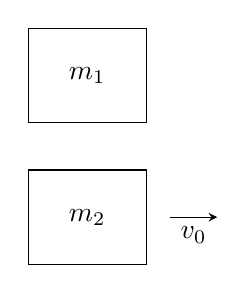
\begin{tikzpicture}[scale=.6, >=stealth]
       \draw  (0,0) rectangle (2.5, 2);
       \draw  (0,3) rectangle (2.5, 5);
    \node at (2.5/2,4){$m_1$};
    \node at (2.5/2,1){$m_2$};
    \draw[->](3,1)--node [below]{$v_0$}(4,1);
    
    \end{tikzpicture}
    \caption{}
    \end{figure}

\begin{solution}    
质量为$m_1$的物体甲做初速度等于零的匀变速直线
运动,经过时间$t$的速度$v_1=\dfrac{F}{m_1}t$。

质量为$m_2$的物体乙做初速度为$v_0$的匀变速直线运动。
经过时间$t$的速度$v_2=v_0+\dfrac{F}{m_2}t$,
由此得
\[v_2-v_1=v_0+\left(\dfrac{F}{m_2}-\dfrac{F}{m_1}\right)t=v_0+\frac{m_1-m_2}{m_1m_2}Ft\]

当$m_1\ge m_2$时,$m_1-m_2\ge 0$, 有$v_2-v_1\ge v_0>0$. 即$v_1$和$v_2$永远不会相等。

当$m_1<m_2$时,有
\[v_2-v_1=v_0-\frac{m_2-m_1}{m_1m_2}Ft\]
令$v_2-v_1=0$, 得
\[t=\frac{m_1m_2v_0}{(m_2-m_1)F}\]
这时有$v_1=v_2$, 即甲乙两物体的速度相等。

说明:由于物体的初速度(等于零)比乙物体的初速度
($v_0$)小,显然,只有甲的加速度比乙的加速度大,即
\[\frac{F}{m_1}>\frac{F}{m_2},\qquad m_1<m_2\]
时,两个物体才能达到相同的速度,这一点,不用公式也可以
得出,借助于公式则可以更明显地看出定量的关系。
\end{solution}
\end{enumerate}

\section{参考资料}
\subsection{研究加速度和力以及质量关系的实验中的误差分析}

在课本实验八和实验九中把砂桶和砂的重量看作使小车
产生加速度的力的条件是:砂桶和砂的质量$m$. 必须远小于小
车的质量$M$. 小车和砂桶应具有相等的加速度,
\[a=\frac{mg}{M+m}\]
式中的$mg$是砂桶和砂的重量,也是作用于由小车和砂桶及
砂组成的物体系的合外力。实验时为了使计算简化,取
$a\approx \dfrac{m}{M}g$。这样就产生了误差,这一误差是由于实验原理的不
完善而带来的,属于系统误差。

下面用具体数字计算一下这一误差的大小。如果实验时
所用小车的质量为200克,砂桶和砂的质量不超过20克,则
加速度的最大值
\[a=\frac{mg}{M+m}=\frac{0.02\x 9.8}{0.2+0.02}=0.89\msq\]
若忽略砂桶和砂的质量$m$, 则
\[a'=\frac{mg}{M}=\frac{0.02\x 9.8}{0.2}=0.98\msq\]
$a'$与$a$相差(即绝对误差)
\[E_a=a'-a=0.98-0.89=0.09\msq\]
相对误差(即百分误差)
\[E_r=\frac{E_a}{a}\x 100\%=\frac{0.09}{0.89}\x 100\%=10.1\%\]

相对误差在10\%左右,这在中学物理实验中是许可的。
当砂桶和砂的质量小于20克,或在小车上加砝码以增大小车
质量时,相对误差均小于10\%, 因此课本上忽略砂桶和砂的
质量来计算加速度的方法是允许的。但是如果砂桶和砂的质
量增大为50克,而小车质量仍为200克,则
\[a=\frac{mg}{M+m}=\frac{0.05\x 9.8}{0.2+0.05}=1.96\msq\]

若忽略$m$, 则
\[a'=\frac{mg}{M}=\frac{0.05\x 9.8}{0.2}=2.45\msq\]
则绝对误差
\[E_a=a'-a=2.45-1.96=0.49\msq\]
相对误差
\[E_r=\frac{E_a}{a}\x 100\%=\frac{0.49}{1.96}\x 100\%=25\%\]
这样的误差就太大了,所以在实验时所用砂桶和砂的质量以
不超过小车质量的1/10为宜.

\subsection{惯性质量和引力质量}
使物体改变运动状态,需要力的作用,在相同的力作用
下,质量越大的物体的加速度越小。这表明了质量是表示物
体所具有的阻碍运动状态改变的一种属性,质量越大,物体越
不容易改变其运动状态,所以质量是物体惯性大小的量度,物
体的这一性质跟物体是否受有重力作用完全无关(譬如放在
水平的气垫导轨上的滑块,或物体在完全失重的情况下)。因
此,牛顿第二定律的公式$F=ma$中所出现的质量$m$, 叫做惯
性质量。

根据万有引力定律可知,物体受到的地球引力的大小和
物体的质量成正比,为了使物体不致由于受到地球引力而掉
向地面,可将物体用绳子悬挂起来(或用支持物支承住)。这样,
绳子(或支持物)就发生形变,物体的质量越大,需要绳子(或
支持物)发生更大程度的形变才能产生足够大的弹力来跟物
体所受到的地球引力相平衡。因此,在这里质量的概念反映了
物体所包含的物质的多少,质量越大,物体所含的物质越多,
受到的地球引力就越大。因此,万有引力定律公式
$F=G\dfrac{Mm}{R^2}$
中所出现的物体质量$m$, 叫做引力质量。

惯性质量和引力质量是从不同的侧面来描述了物质的属
性,它们之间存在着怎样的关系呢?

设有$A,B$两个物体,它们的惯性质量分别为$m_A$、$m_B$, 引
力质量分别为$m'_A$、$m'_B$. 把$A$、$B$这两个物体放在地球上的
同一地点,则它们所受到的地球引力分别为:
\[F_A=G\frac{Mm'_A}{R^2}=G_A,\qquad F_B=G\frac{Mm'_B}{R^2}=G_B\]

若将以上两式相比,则得:
\begin{equation}
    \frac{G_A}{G_B}=\frac{m'_A}{m'_B}
\end{equation}
这表明了$A$、$B$物体所受重力的比等于它们的引力质量的比。

如果使$A$、$B$物体在重力的作用下自由下落,则根据牛顿
第二定律可知,$G_A=m_Ag_A$; $G_B=m_Bg_B$。

由于在同一地点,重力加速度都相等,即$g_A=g_B=g$. 于
是:
\begin{equation}
    \frac{G_A}{G_B}=\frac{m_A}{m_B}
\end{equation}

这表明了在地球上同一地点,物体的重量的比等于它们
的惯性质量的比。

比较(3.1)式和(3.2)式,可见物体的惯性质量$m$和引力质量
$m'$是一致的。

对单摆的振动加以讨论,也可以得出惯性质量和引力质
量是等效的结论。单摆振动在偏角很小的情况下,可看作是
有简谐振动,对于简谐振动来说,它的周期$T=2\pi\sqrt{\frac{m}{k}}$, 
式中$m$是振动系统的惯性质量,$k$是决定于振动系统的一个常数。
在单摆这一振动系统中,$k=\dfrac{m'}{\ell}g$,式中$m'$是摆球的引力质量.
代入周期公式,得单摆振动的周期公式
\[T=2\pi\sqrt{\frac{m\ell}{m'g}}\]

从实验证明,在摆角很小时,单摆的振动周期跟摆长l的
平方根成正比,跟所在地点的重力加速度$g$的平方根成反比,
而与物体质量无关,即
$$T=2\pi\sqrt{\frac{\ell}{g}}$$
这只有认为$m'=m$的情
况下才是可能的,因此物体的惯性质量和引力质量是等效的。

因此,在中学物理教学中,不必区分惯性质量和引力质量。


\subsection{狭义相对论和经典力学}
以牛顿定律为基础的经典力学认为,物体的长度和时间
间隔跟物体运动的速度没有关系,即把空间和时间看成是绝
对的。经典力学还认为物体的质量跟物体运动的速度大小也
是无关的。这些结论对于研究宏观物体的运动无疑是正确的,
跟人们的日常经验也是一致的。

但在研究微观粒子的高速运动时,发现了用经典力学无
法解释的矛盾.爱因斯坦在1905年发表了《论运动物体的电
动力学》的著名论文,提出狭义相对性原理(即第一个假设:在
所有惯性系中物理定律具有相同的形式,没有一个惯性系比
别的惯性系更优越)和光速不变原理(即第二个假设:在所有
惯性系中光速都是相同的),创立了狭义相对论,可以用来处
理微观粒子的高速运动的问题。

狭义相对论指出:有两个惯性系$s$和$s'$, 它们具有互相平
行的坐标轴$(x,y,z)$, 并且$x$-$x'$轴是公共的.若$s'$相对于$s$
以速率$v$运动,在这两个不同的惯性系中的观察者,对于同一
地点发生的两个事件之间的时间间隔的测量结果是不同的。
在$s'$中的观察者测得的时间间隔为$\Delta t'$, 而由于$s$中的观察
者认为$s'$是在运动着的,他所测得的时间间隔$\Delta t$由下式
给出:
\[\Delta t=\frac{\Delta t'}{\sqrt{1-\left(\dfrac{v}{c}\right)^2}}\]

可见$\Delta t>\Delta t'$. 即时间发生了“膨胀”,运动的钟变慢
了——通常叫做钟慢效应。

如果有一根相对于$s'$是静止的尺,平行于$x'$轴放置,在
$s'$中测得尺的长度为$\Delta x'$, 而在$s$中的观察者看来,这把尺是
运动的,他测得的尺的长度$\Delta x$由下式给出:
\[\Delta x={\sqrt{1-\left(\dfrac{v}{c}\right)^2}}\Delta x'\]

可见$\Delta x<\Delta x'$, 即长度发生了“收缩”,运动的尺变短
了——通常叫做尺缩效应。

狭义相对论还导出,跟对时间间隔和长度的测量一样,质
量$m$也是速率$v$的函数。如果质点静止时的质量为$m_0$, 则
质点相对于观察者以速率$v$运动时,它的相对论质量$m$将由
下式给出:
\[m=\frac{m_0}{\sqrt{1-\left(\dfrac{v}{c}\right)^2}}\]

可见$m>m_0$, 即质量随着速率的增大而变大,通常叫做
质-速关系。

以上三个关系式表明了狭义相对论提出的一种新的时空
观。而当速率$v\ll c$时,则$\Delta t\approx \Delta t'$, $\Delta x\approx \Delta x'$, $m\approx m_0$. 这表
明经典力学所描述的运动规律是狭义相对论的特殊情况。因
而处理宏观物体的低速运动时使用牛顿力学是足够准确的。

此外,从狭义相对论的结论中,还导出了质量和能量的等
效原理。
\[E=mc^2\]

这表明了总能量守恒和相对论质量守恒是等效的,这一
原理是研究原子核反应及其应用的一个重要理论依据。
